% !TeX root = text.tex
\documentclass{template/socthesis}

\usepackage{subcaption}
\usepackage{amsmath}
\usepackage{enumitem}

% my own code
\usepackage{xkvltxp}

\usepackage[skip=10pt plus1pt, indent=0pt]{parskip}
\usepackage[czech]{babel}

\usepackage[nomargin, inline, marginclue, author=,status=draft]{fixme}
\makeatletter
\renewcommand*\FXLayoutInline[3]{%
  {\@fxuseface{inline}\ignorespaces[#2]}}
\makeatother


%%%%%% podbarvení bloků kódu / vygenerovaných ai
\usepackage{xcolor}
\usepackage{listings}
\usepackage{tcolorbox}

\tcbuselibrary{breakable}

\definecolor{aiblue}{rgb}{127,127,255}
\definecolor{aibackground}{rgb}{100,100,100}

\lstdefinestyle{aistyle}{
    backgroundcolor=\color{aibackground},   
    commentstyle=\color{aiblue},
    keywordstyle=\color{aiblue},
    numberstyle=\tiny\color{aiblue},
    stringstyle=\color{aiblue},
    basicstyle=\ttfamily\footnotesize,
    breakatwhitespace=false,         
    breaklines=true,                 
    captionpos=b,                    
    keepspaces=true,                 
    numbers=left,                    
    numbersep=5pt,                  
    showspaces=false,                
    showstringspaces=false,
    showtabs=false,                  
    tabsize=2
}

\definecolor{codegreen}{rgb}{0,0.6,0}
\definecolor{codegray}{rgb}{0.5,0.5,0.5}
\definecolor{codepurple}{rgb}{0.58,0,0.82}
\definecolor{backcolour}{rgb}{0.95,0.95,0.92}

\lstdefinestyle{code}{
    backgroundcolor=\color{backcolour},   
    commentstyle=\color{codegreen},
    keywordstyle=\color{magenta},
    numberstyle=\tiny\color{codegray},
    stringstyle=\color{codepurple},
    basicstyle=\ttfamily\footnotesize,
    breakatwhitespace=false,         
    breaklines=true,                 
    captionpos=b,                    
    keepspaces=true,                 
    numbers=left,                    
    numbersep=5pt,                  
    showspaces=false,                
    showstringspaces=false,
    showtabs=false,                  
    tabsize=2
}
% languages
\definecolor{lightgray}{rgb}{0.95, 0.95, 0.95}
\definecolor{darkgray}{rgb}{0.4, 0.4, 0.4}
%\definecolor{purple}{rgb}{0.65, 0.12, 0.82}
\definecolor{editorGray}{rgb}{0.95, 0.95, 0.95}
\definecolor{editorOcher}{rgb}{1, 0.5, 0} % #FF7F00 -> rgb(239, 169, 0)
\definecolor{editorGreen}{rgb}{0, 0.5, 0} % #007C00 -> rgb(0, 124, 0)
\definecolor{orange}{rgb}{1,0.45,0.13}		
\definecolor{olive}{rgb}{0.17,0.59,0.20}
\definecolor{brown}{rgb}{0.69,0.31,0.31}
\definecolor{purple}{rgb}{0.38,0.18,0.81}
\definecolor{lightblue}{rgb}{0.1,0.57,0.7}
\definecolor{lightred}{rgb}{1,0.4,0.5}
\usepackage{upquote}
\usepackage{listings}
% CSS
\lstdefinelanguage{CSS}{
  keywords={color,background-image:,margin,padding,font,weight,display,position,top,left,right,bottom,list,style,border,size,white,space,min,width, transition:, transform:, transition-property, transition-duration, transition-timing-function},	
  sensitive=true,
  morecomment=[l]{//},
  morecomment=[s]{/*}{*/},
  morestring=[b]',
  morestring=[b]",
  alsoletter={:},
  alsodigit={-}
}

% JavaScript
\lstdefinelanguage{JavaScript}{
  morekeywords={typeof, new, true, false, catch, function, return, null, catch, switch, var, if, in, while, do, else, case, break},
  morecomment=[s]{/*}{*/},
  morecomment=[l]//,
  morestring=[b]",
  morestring=[b]'
}

\lstdefinelanguage{HTML5}{
  language=html,
  sensitive=true,	
  alsoletter={<>=-},	
  morecomment=[s]{<!-}{-->},
  tag=[s],
  otherkeywords={
  % General
  >,
  % Standard tags
	<!DOCTYPE,
  </html, <html, <head, <title, </title, <style, </style, <link, </head, <meta, />,
	% body
	</body, <body,
	% Divs
	</div, <div, </div>, 
	% Paragraphs
	</p, <p, </p>,
	% scripts
	</script, <script,
  % More tags...
  <canvas, /canvas>, <svg, <rect, <animateTransform, </rect>, </svg>, <video, <source, <iframe, </iframe>, </video>, <image, </image>, <header, </header, <article, </article
  },
  ndkeywords={
  % General
  =,
  % HTML attributes
  charset=, src=, id=, width=, height=, style=, type=, rel=, href=,
  % SVG attributes
  fill=, attributeName=, begin=, dur=, from=, to=, poster=, controls=, x=, y=, repeatCount=, xlink:href=,
  % properties
  margin:, padding:, background-image:, border:, top:, left:, position:, width:, height:, margin-top:, margin-bottom:, font-size:, line-height:,
	% CSS3 properties
  transform:, -moz-transform:, -webkit-transform:,
  animation:, -webkit-animation:,
  transition:,  transition-duration:, transition-property:, transition-timing-function:,
  }
}

\lstdefinestyle{htmlcssjs} {%
  % General design
%  backgroundcolor=\color{editorGray},
  basicstyle={\footnotesize\ttfamily},   
  frame=b,
  % line-numbers
  xleftmargin={0.75cm},
  numbers=left,
  stepnumber=1,
  firstnumber=1,
  numberfirstline=true,	
  % Code design
  identifierstyle=\color{black},
  keywordstyle=\color{blue}\bfseries,
  ndkeywordstyle=\color{editorGreen}\bfseries,
  stringstyle=\color{editorOcher}\ttfamily,
  commentstyle=\color{brown}\ttfamily,
  % Code
  language=HTML5,
  alsolanguage=JavaScript,
  alsodigit={.:;},	
  tabsize=2,
  showtabs=false,
  showspaces=false,
  showstringspaces=false,
  extendedchars=true,
  breaklines=true,
  % German umlauts
  literate=%
  {Ö}{{\"O}}1
  {Ä}{{\"A}}1
  {Ü}{{\"U}}1
  {ß}{{\ss}}1
  {ü}{{\"u}}1
  {ä}{{\"a}}1
  {ö}{{\"o}}1
}
%
\lstdefinestyle{py} {%
language=python,
literate=%
*{0}{{{\color{lightred}0}}}1
{1}{{{\color{lightred}1}}}1
{2}{{{\color{lightred}2}}}1
{3}{{{\color{lightred}3}}}1
{4}{{{\color{lightred}4}}}1
{5}{{{\color{lightred}5}}}1
{6}{{{\color{lightred}6}}}1
{7}{{{\color{lightred}7}}}1
{8}{{{\color{lightred}8}}}1
{9}{{{\color{lightred}9}}}1,
basicstyle=\footnotesize\ttfamily, % Standardschrift
numbers=left,               % Ort der Zeilennummern
%numberstyle=\tiny,          % Stil der Zeilennummern
%stepnumber=2,               % Abstand zwischen den Zeilennummern
numbersep=5pt,              % Abstand der Nummern zum Text
tabsize=4,                  % Groesse von Tabs
extendedchars=true,         %
breaklines=true,            % Zeilen werden Umgebrochen
keywordstyle=\color{blue}\bfseries,
frame=b,
commentstyle=\color{brown}\itshape,
stringstyle=\color{editorOcher}\ttfamily, % Farbe der String
showspaces=false,           % Leerzeichen anzeigen ?
showtabs=false,             % Tabs anzeigen ?
xleftmargin=17pt,
framexleftmargin=17pt,
framexrightmargin=5pt,
framexbottommargin=4pt,
%backgroundcolor=\color{lightgray},
showstringspaces=false,      % Leerzeichen in Strings anzeigen ?
}%
%

% https://tex.stackexchange.com/questions/24528/having-problems-with-listings-and-utf-8-can-it-be-fixed
\lstset{style=aistyle,
inputencoding=utf8,
extendedchars=true,
literate=%
{á}{{\'a}}1
{č}{{\v{c}}}1
{ď}{{\v{d}}}1
{é}{{\'e}}1
{ě}{{\v{e}}}1
{í}{{\'{\i}}}1
{ň}{{\v{n}}}1
{ó}{{\'o}}1
{ř}{{\v{r}}}1
{š}{{\v{s}}}1
{ť}{{\v{t}}}1
{ú}{{\'u}}1
{ů}{{\r{u}}}1
{ý}{{\'y}}1
{ž}{{\v{z}}}1
{Á}{{\'A}}1
{Č}{{\v{C}}}1
{Ď}{{\v{D}}}1
{É}{{\'E}}1
{Ě}{{\v{E}}}1
{Í}{{\'I}}1
{Ň}{{\v{N}}}1
{Ó}{{\'O}}1
{Ř}{{\v{R}}}1
{Š}{{\v{S}}}1
{Ť}{{\v{T}}}1
{Ú}{{\'U}}1
{Ů}{{\r{U}}}1
{Ý}{{\'Y}}1
{Ž}{{\v{Z}}}1
}

\DeclareUnicodeCharacter{2212}{\textminus}% requires a unicode capable editor

\addbibresource{text.bib}

\titlecz{Laserový projektor}
\titleen{Laser projector}
\author{Šimon Hrouda}
\field{10}
\school{Gymnázium Brno-Řečkovice}
\exmentor{Tomáš Rohlínek}
\exmentorstatement{Tomáše Rohlínka}
\inmentor{Mgr. Kateřina Vídenková}
\inmentorstatement{Mgr. Kateřiny Vídenkové}

% Změňte, pokud se liší
%\region{Jihomoravský}
\placefooter{Brno 2024}

\begin{document}
% \newcommand{\bard-gen}[3]{text vygenerován ai #1}
\newcommand{\bardgen}[3]{following text generated by ai (google bard) on #1\\%
  \begin{tcolorbox}[breakable, colback=blue!20]
    #2
  \end{tcolorbox}
  \begin{tcolorbox}[breakable, colback=blue!10, colframe=white]
    #3
  \end{tcolorbox}
}


\maketitle

\makecopyrightstatement{V~Brně}

\makethanks{Děkuji svému externímu konzultantovi Tomáši Rohlínkovi a své interní konzultantce Mgr. Kateřině Vídenkové za obětavou pomoc, podnětné připomínky a nekonečnou trpělivost, kterou mi během práce poskytovali.}

\pagestyle{empty}

\section*{Anotace}


\subsection*{Klíčová slova}


\vspace{20mm}

\section*{Annotation}


\subsection*{Keywords}


\newpage
\pagestyle{plain}

\tableofcontents % vysází obsah

%%% Začátek práce
\setcounter{figure}{0}
\setcounter{table}{0}
\newpage

\fxnote{TODO 3. osoba - Práce se zaměřuje}
https://www.sciencedirect.com/search?qs=galvanometer
muzu rict, ze jsem neco nezvladl dohledat :)

\chapter*{Úvod}
\addcontentsline{toc}{chapter}{Úvod} % přidá položku úvod do obsahu
V této práci se zaměřuji na návrh a výrobu laserového projektoru, který bude za pomoci páru zrcátek připevněných na galvanometrech rychle měnit směr laserového paprsku a tím vykreslovat obraz na promítací plochu.

Laser scanning je vyuzivan v mnoha oblastech, například  v brýlích pro rozšířenou realitu nebo v Heads Up Displejích pro piloty. \fxnote{TODO: ozdrojovat využití laserscanningu}
+3d scanning/modeling (height mapping) \url{https://theses.hal.science/tel-00682442}
V této  práci jsem se proto rozhodl pro tuto technologii vytvořit jednoduché uživatelské prostředí, ve kterém si i začínající kutil může vyzkoušet jak funguje.

\newpage

definice pojmů a zkratek
\begin{center}
  \begin{tabular}{c c c}
    CLGS & Closed Loop Galvanometer System & systém galvanometru se zpětnou vazbou \\
    OLGS & Open Loop Galvanometer System   & systém galvanometru bez zpětné vazby  \\
    SPI  & Serial Peripheral Interface     & sériové periferní rozhraní            \\
  \end{tabular}
\end{center}

\chapter{hardware}

\section{Raspberry Pi}

\section{Galvanometr a zrcátko}
\begin{itemize}
  \item
        Galvanometry, často nazývané galva, jsou elektronické součástky používané k měření intenzity a směru elektrického proudu. \cite{galvo}

        Můžeme je rozdělit mezi galvanometry s uzavřenou smyčkou zpětné vazby (CLGS) a galvanometry bez uzavřené smyčky zpětné vazby (OLGS). \cite{how-ls-work}
        % Druhé zmíňěné mají velice specifické využití - barcode scanners a jsou zdokumentované pouze ve zdroji .

        \cite{advanced-galvo}
        ale postupně nachází uplatnění ve více a více odvětvích práce s lasery.
        Oproti jiným možnostem nabízí flexibilitu, rychlost a přesnost za nízkou cenu.


        V této práci jsou ale využívány CLGS, které jsou lépe zdokumentované.

        V CLGS jsou potřeba 3 hlavní prvky, %pohybový akční člen, senzor a kontrolní desku - vycucáno z prstu

        Nejmodernější galvanometrové polohovací systémy jsou založené na principech elektromotorů s permanentními magnety, kde
        \cite{advanced-galvo}
  \item
        \url{https://en.wikipedia.org/wiki/Galvanometer}\\
        \url{https://en.wikipedia.org/wiki/Laser_scanning}\\
        \url{https://en.wikipedia.org/wiki/Mirror_galvanometer}\\
        \url{https://en.wikipedia.org/wiki/Laser_lighting_display}

        A mirror galvanometer is an ammeter that indicates it has sensed an electric current by deflecting a light beam with a mirror.
        The mirror galvanometer consists of a long fine coil of silk-covered copper wire. %wtf silk == hedvábí??
        In the heart of that coil, within a little air-chamber, a small round mirror is hung by a single fibre of floss silk, with four tiny magnets cemented to its back
        The small weight of the mirror and magnets which form the moving part of this instrument, and the range to which the minute motions of the mirror can be magnified on the screen by the reflected beam of light, which acts as a long impalpable hand or pointer, render the mirror galvanometer marvellously sensitive to the current, especially when compared with other forms of receiving instruments.

        Zrcadlový galvanometr je měřič proudu, který reaguje na měřený proud vychýlením světelného paprsku zrcátkem připevněném na jeho konci.
        % Skládá se z dlouhé  tenké cívky měděného drátu potaženého hedvábím %wtf silk == hedvábí??
        % Ve středu této cívky je v malé vzduchové komůrce na jediném vláknu hedvábí

        Skládá se z cívky a
        \cite{zrcadlovy-galvanometr-wiki}

  \item
        \bardgen{2023-10-20}{popiš mi jak je sestaven a jak funguje galvanometr se zrcátkem k odrážení světelného paprsku}{
          Galvanometr se zrcátkem je sestaven z následujících komponent:

          * **Cívka:** Cívka je navinuta na jádře z feromagnetického materiálu, jako je železo nebo nikl. Cívkou prochází elektrický proud, který vytváří magnetické pole.
          * **Ukazatel:** Ukazatel je připojen k cívce a je vyroben z lehkého materiálu, jako je hliník nebo plast. Ukazatel je vychýlen magnetickým polem vytvářeným cívkou.
          * **Zrcátko:** Zrcátko je připojeno k ukazateli a odráží světelný paprsek.
          * **Okulár:** Okulár je umístěn tak, aby bylo možné pozorovat odraz světelného paprsku.

          **Jak funguje:**

          Když prochází cívkou elektrický proud, vytváří magnetické pole. Toto magnetické pole působí na ukazatel a vychýlí ho. Velikost výchylky ukazatele je přímo úměrná velikosti proudu procházejícího cívkou.

          Zrcátko je připojeno k ukazateli a odráží světelný paprsek. Když se ukazatel vychýlí, odraz světelného paprsku se také vychýlí.

          Okulár je umístěn tak, aby bylo možné pozorovat odraz světelného paprsku. Velikost vychýlení světelného paprsku je přímo úměrná velikosti proudu procházejícího cívkou.

          **Výhody:**

          * Galvanometr se zrcátkem je citlivější než galvanometr bez zrcátka.
          * Galvanometr se zrcátkem lze použít k měření velmi malých proudů.

          **Nevýhody:**

          * Galvanometr se zrcátkem je dražší než galvanometr bez zrcátka.

          **Použití:**

          Galvanometr se zrcátkem se používá k měření velmi malých proudů. Používá se například v elektrotechnice, lékařství a fyzice.
        }
\end{itemize}

ovládá se variabilním proudem

\section{hlavice}
\href{https://elenlaser.com/blog/galvo-head-laser-focus-tool.html}{The mirrors, mounted perpendicularly on the engines, move the laser beam along the X and Y axes according to the input received from the motor.
The big advantage of these devices is that they can reach a very high acceleration and speed of}
well asi patří do sekce galvanometr

\section{moje deska na napětí}
Galvanometry v obou osách pohybu potřebujeí analogový vstupní signál v rozpětí $-15$~V až $+15$~V udávající vychýlení galvanometru v daném směru.

Vytváření tohoto signálu jsem rozdělil do dvou částí, nejdříve pomocí DAC (digital-to-analog converter, D/A převodník) připojeného k RPi vytvořím signál v rozpětí 0 až 5~V a následně tento signál pomocí operačního zesilovače převedu na požadované rozpětí.
Celé zapojení je vidět na obrázku \ref{fig:dac_board}
\begin{figure}[!htb]
  \centering
  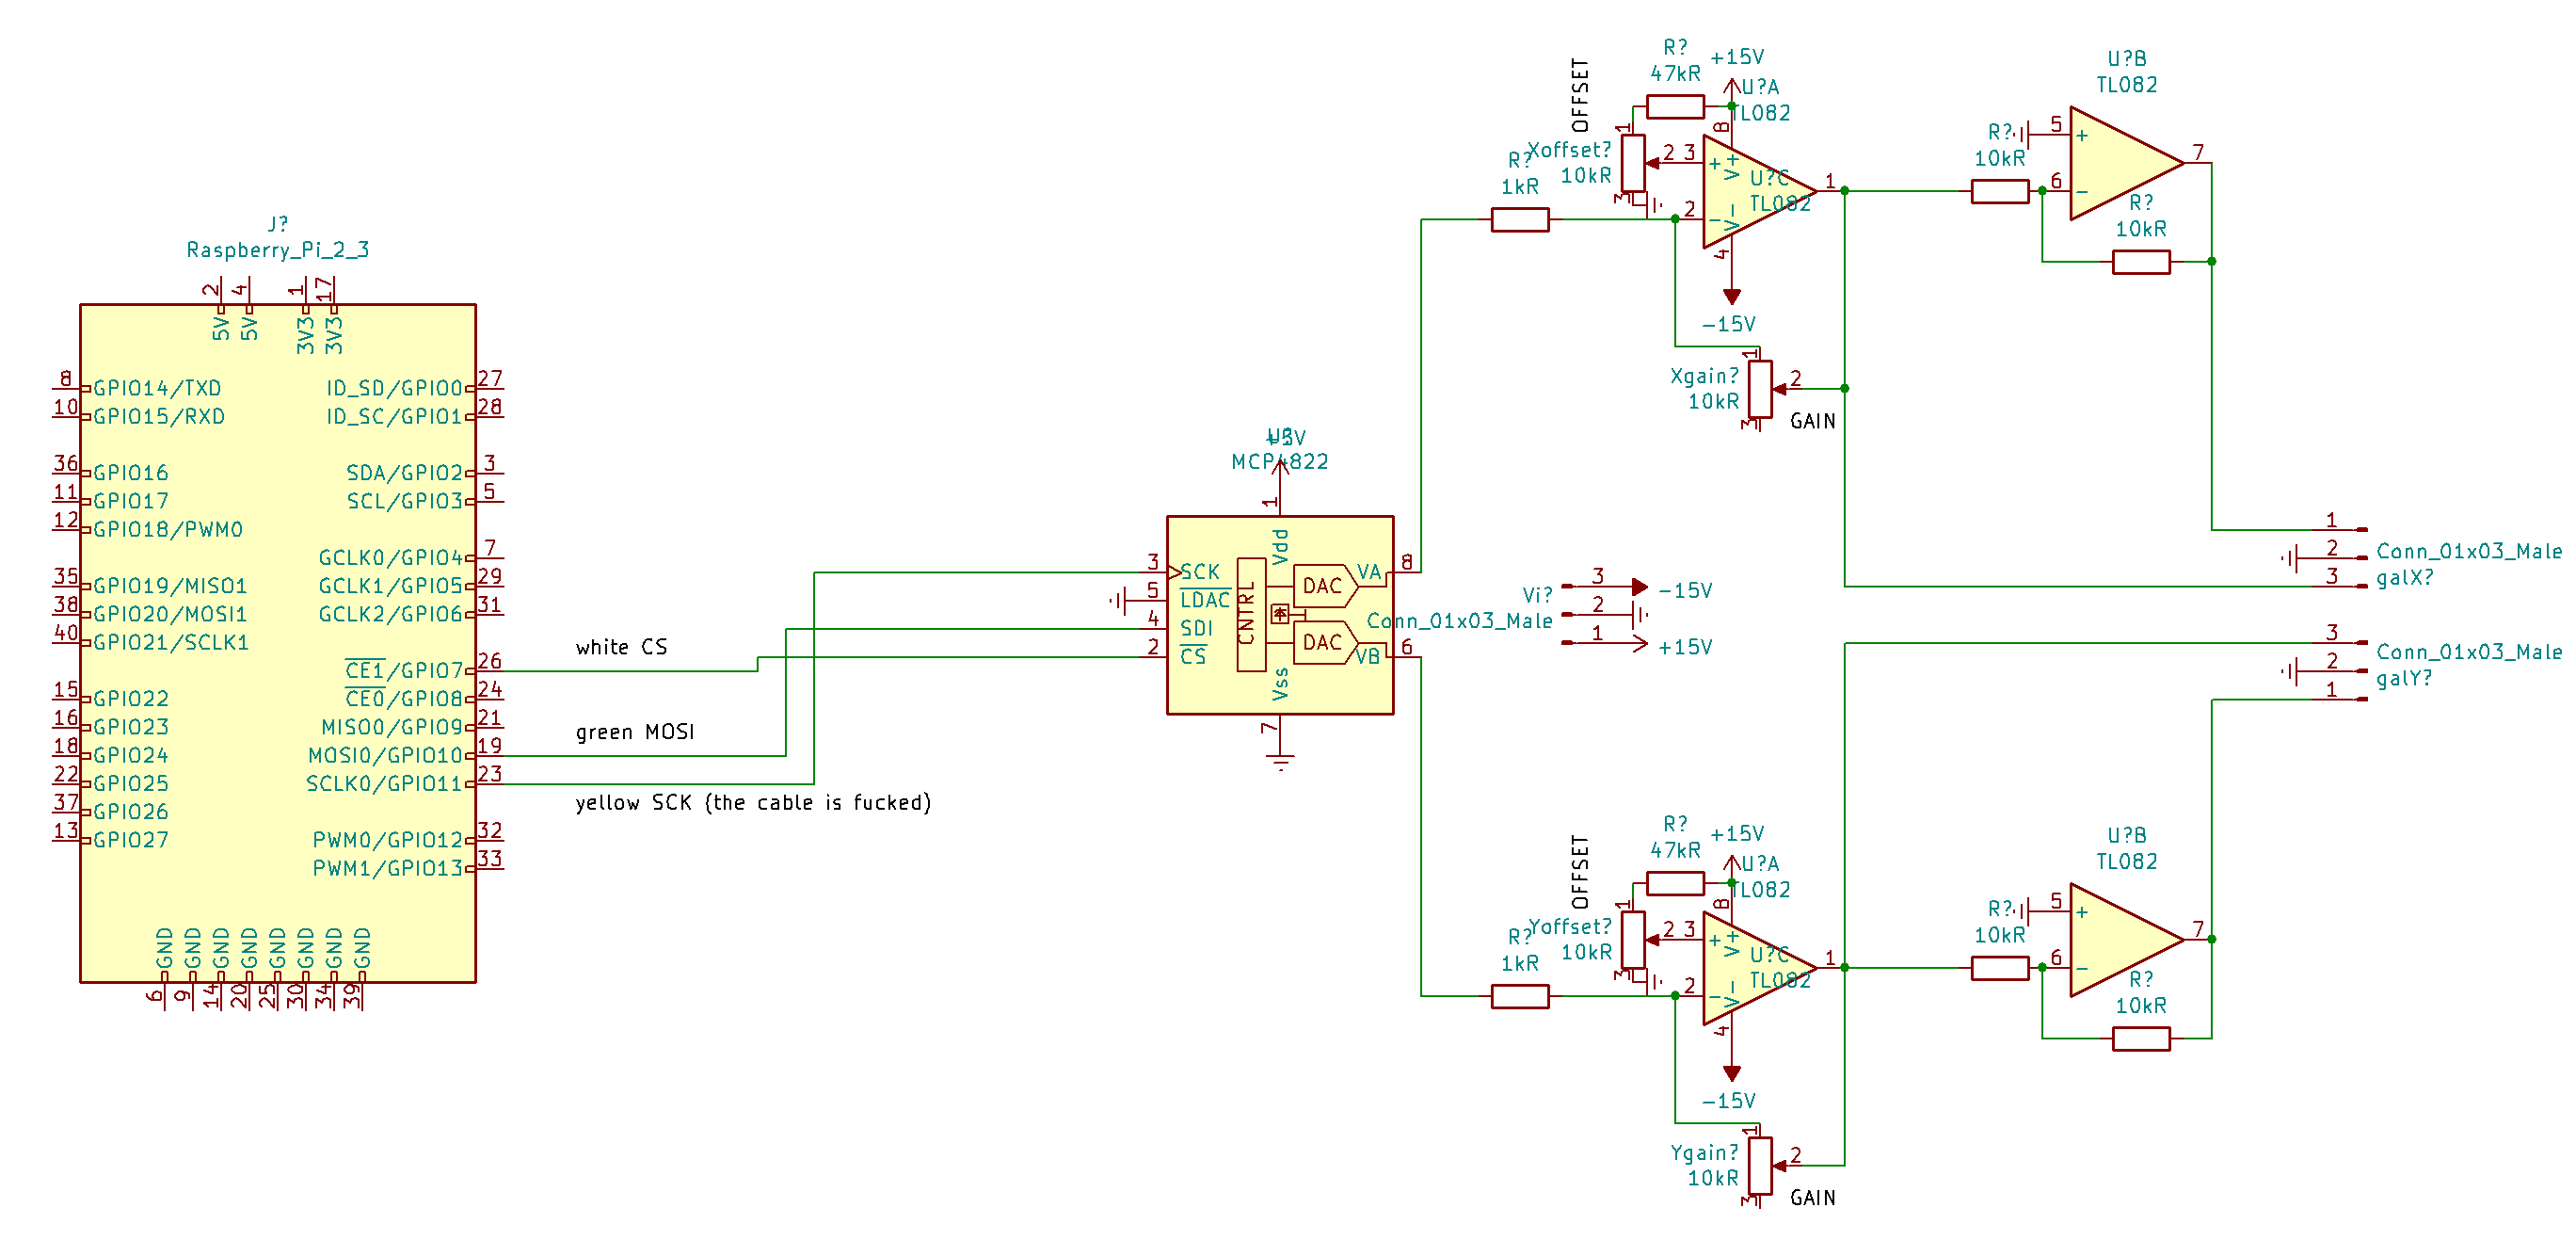
\includegraphics[width=1\textwidth]{img/dac_board.png} %unreadable text, make schem more compact
  \caption{\label{fig:dac_board}Zapojení DAC a zesilovačů k RPi a řídící desce galvanometrů}
\end{figure}

\subsection{dac}
K generování signálu v rozpětí 0--5~V jsem využil DAC MCP4822 od firmy \href{https://www.microchip.com}{Microchip Technology Inc.}\ \fxnote{TODO tečka? ("\textbackslash " == explicitni mezera)}
Tento čip podporuje komunikaci přes rozhraní SPI, pracuje s napájecím napětím 5~V a s 12bitovým rozlišením (je schopen vygenerovat 4~096 různých napětí) na dvou kanálech.

Komunikace mezi RPi a čipem je zprostředkována rozhraním SPI, toto rozhraní využívám pomocí knihovny ze serveru \url{https://github.com}\footnote{\url{https://github.com/pawel-kusinski/mcp4822-linux}; staženo 28.~12.~2023} \fxnote{TODO tečka?} \fxnote{FIXME pouzivam jinou knihovnu, bundled with lasershow}
\fxnote{TODO more spec}
Tato knihovna poskytuje funkce \lstinline[language=C]!bool mcp4822_initialize();bool mcp4822_set_voltage(mcp4822_channel_t channel, uint16_t value_mV);void mcp4822_deinitialize();!, se kterými pracuji v mém kódu.
\subsection{amps}
K rozšíření signálu z DAC jsem využil dva operační zesilovače TL082 od firmy \href{https://www.ti.com/}{Texas Instruments Incorporated}. Každý z nich je připojený na jeden kanál DAC čipu mcp4822.
\fxnote{TODO more spec}
Tyto čipy mi napěťové rozpětí zvýší z 0--5~V na $-15$~V až $+15$~V.

\section{laser}
\section{if rgb: 3 dacs}


\fxnote{TODO cos udelal svyho vlastne a jak to facha}

\section{napájení}
\fxnote{TODO ay tak co, zvladls to dat na baterky?}

\chapter{software} \fxnote{TODO: zkrátit věty}
Tento laserový projektor se skládá ze dvou částí. Jednou je software pro řízení galvanometrů a druhou je software pro interakci s uživatelem.

O řízení galvanometrů se stará program lasershow, který je psaný v jazyce c++ pro maximální rychlost. Tento program běží na pozadí a čeká na příkazy od programů určených k interakci s uživatelem. Na tento program se zaměřuje kapitola lasershow. \fxnote{TODO: odkaz}

Dále jsou tu programy, které se starají o interakci s uživatelem. Tyto programy přijímají příkazy od uživatele a posílají je programu lasershow. Navíc od lasershow získávají výstup, který následně zprostředkovávají uživateli; důkladněji popsáno v kapitole \ref{comms}.

Mezi tyto programy patří programy UI, web\_ui a discord\_bot. Program UI spravuje OLED displej, přijímá od uživatele vstup rotačním enkodérem a je psaný v c++ pro jednodušší interakci s hardwarem. Program web\_ui využívá runtime Node.js, ve kterém je nenáročné vytvořit http server dostupný z lokální sítě. \fxnote{(A)?} Program discord\_bot, také využívající Node.js, přijímá příkazy z chatovací aplikace discord a je přístupný i přes internet.

Nakonec je tu program wifi\_manager, ten spravuje wifi připojení RPi, je psaný v Node.js a komunikuje s programy, které interagují s uživatelem stejně jako program lasershow.

\section{komunikace mezi programy} \label{comms}
Všechny tyto programy jsou propojeny síťovými sockety zprostředkovanými knihovnou ZeroMQ, která nabízí frontu\footnote{Ve frontě jsou zprávy seřazeny od té nejdříve odeslané.} zpráv, bez potřeby samostatně běžícího brokeru.\fxnote{TODO: divna jednicka}

Tato knihovna je využita k vytvoření dvou socketů, jedním lasershow přijímá příkazy od uživatele prostřednictvím ostatních programů (vstupní socket na portu 5557, viz obr. \ref{fig:tcp5557}) a do druhého posílá informace ostatním programům (výstupní socket na portu 5556, viz obr. \ref{fig:tcp5556}), aby je zprostředkovaly uživateli. Do prvního zmíněného posílají progamy interagující s uživatelem příkazy pro programy lasershow a wifi\_manager. Do druhého posílá lasershow informace o stavu a změnách nastavení  a také wifi\_manager informace o stavu a změnách v nastavení WiFi.

Příkazy pro programy lasershow a wifi\_manager vypadají následovně
\fxnote{TODO: příklady příkazů pro lasershow a wifi\_manager z \url{https://github.com/phuid/laser_projector/blob/master/README.md}}
\fxnote{TODO: příklady status infos od lasershow a wifi\_manager z \url{https://github.com/phuid/laser_projector/blob/master/README.md}}

\begin{figure}[!htb]
  \centering
  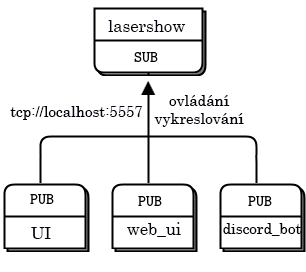
\includegraphics[width=0.5\textwidth]{img/tcp5557.png}
  \caption{\label{fig:tcp5557}komunikace mezi programy vstupním socketem na portu 5557}
\end{figure}
\begin{figure}[!htb]
  \centering
  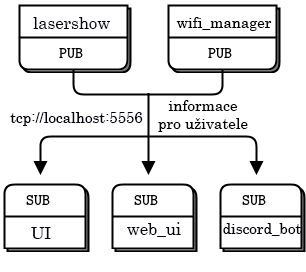
\includegraphics[width=0.5\textwidth]{img/tcp5556.png}
  \caption{\label{fig:tcp5556}komunikace mezi programy výstupním socketem na portu 5556}
\end{figure}

\section{lasershow exec}

Program lasershow je psaný v jazyce c++, který je kompilovaný a obecně považovaný za jeden z nejrychlejších jazyků. Druhé zmíněné se hodí, jelikož chceme vykreslovat co možná nejrychleji.

Tento program zaregistruje vstupní TCP socket na portu 5557 a knihovnou ZeroMQ se na něm přihlásí k odběru zpráv, které do něj publikují ostatní programy. Zárověn podobně zaregistruje výstupní socket na portu 5556, do kterého později bude posílat zprávy pro programy, které interagují s uživatelem.

Následně se připojí k DAC a čeká na zprávy od ostatních programů. Jakmile zprávu obdrží, zpracuje ji a pokud je požadována změna nastavení, okamžitě ji provede a aktuální nastavení si uloží do souboru, jestliže je požadováno vykreslení obrazu ze souboru, začne obraz vykreslovat. Při tom průběžně posílá informace o stavu vykreslování do výstupního socketu. I při vykreslování obrazu tento program zpracovává zprávy a pokyny ze vstupního socketu.

Část tohoto programu, která komunikuje s DAC, je převzatá z projektu \url{https://github.com/tteskac/rpi-lasershow}\footnote{staženo 28.~12.~2023}, z tohoto projektu je převzatá i část, která čte ILDA soubory, ale ta byla v rámci této práce upravena, pro podporu barevných obrazů k vykreslení.

\fxnote{TODO: diagram programu}

\fxnote{TODO: priklad zmq}

\lstinputlisting[language=c++, style=code]{code_examples/zmq_server.cpp}
\lstinputlisting[language=c++, style=code]{code_examples/zmq_client.cpp}

\section{UI}

Program UI je také psaný v jazyce c++ a využívá knihovnu WiringPi, která umožňuje jednoduchou komunikaci s GPIO piny Raspberry Pi. Tento program ovládá OLED displej, který je připojený na Raspberry Pi pomocí rozhraní I2C, a přijímá vstup od uživatele čtením rotačního enkodéru s tlačítkem.

Program se při začátku exekuce pomocí knihovny ZeroMQ přihlásí ke vstupnímu socketu a k odběru zpráv z výstupního TCP socketu, kam publikuje zprávy o stavu vykreslování program lasershow. Dále si pomocí knihovny wiringPi zaregistruje zpracovávání přerušení z enkodéru a tlačítka na něm a čeká buď na interakci s uživatelem, který by skrz něj poslal zprávy programu lasershow, nebo na zprávy od lasershow, které by zobrazil uživateli.

\fxnote{TODO: diagram programu}

\section{web\_ui}

Narozdíl od předchozích dvou zmiňovaných programů je program web\_ui psaný v jazyce javascript, ten nepatří mezi nejrychlejší, ale díky runtime Node.js a knihovnám http a formidable v něm bylo časově nenáročné vytořit http web server.

Tento server běží na portu 3000 a je dostupný z lokální sítě (tzn. přímo z\ Raspberry Pi na adrese http://localhost:3000 nebo z jakéhokoliv zařízení na stejné lokální síti na adrese http://IP\_ADRESA\_RPI:3000).
Program je využíván pro jednoduchou interakci s uživatelem, který může pomocí webového prohlížeče ovládat laserový projektor pár kliknutími i zadávat vlastní příkazy klávesnicí.

\fxnote{TODO: příklad http serveru}
\lstinputlisting[language=JavaScript, style=code]{code_examples/http_static_files.js}

Stejně jako program UI za pomoci knihovny ZeroMQ tento program odebírá z výstupního socketu zprávy o průběhu vykreslování od programu lasershow a odesílá mu pokyny uživatele na vstupní socket.

\fxnote{TODO: příklad přihlášení k socketům v js}

\fxnote{TODO: xterm + ssh}

\section{discord bot}

Posledním programem, který je využíván k interakci s uživatelem je discord\_bot, který je také psaný v jazyce javascript v runtime Node.js, stejně jako předchozí programy se přihlásí k socketům knihovnou zmq, ale na rozdíl od nich tento program může interagovat s uživatelem přes internet ať už je kdekoliv na světě.
Pomocí knihovny discord.js se přihlásí k předem vytvořenému bot účtu, který může na předem vytvořeném discord serveru čekat na zprávy od uživatele, ty posílat do vstupního socketu a posílat uživateli zpětnou vazbu, kterou příjme z výstupního socketu.

\section{wifi\_manager}

V rámci této práce byl vyvinut ještě jeden program, který se přímo nepodílí ani na projekci, ani na interakci s uživatelem.

Program wifi\_manager je také napsaný v jazyce JavaScript s využitím runtime Node.js. Registruje se ke stejným socketům jako lasershow, přijímá příkazy týkající se nastavení WiFi na Raspberry Pi TCP socketem na portu 5557 a odesílá zpětnou vazbu na TCP socket s portem 5556.

\fxnote{TODO: jak se komunikace s lasershow odlisuje od wifi\_managera}

\fxnote{TODO: ukazka(idk what)}

Hlavním úkolem tohoto programu je správa a konfigurace WiFi připojení na Raspberry Pi. Přijímá příkazy od ostatních programů a nastavuje WiFi parametry na základě těchto příkazů. Tím umožňuje uživatelům snadno a pohodlně nastavit WiFi připojení na svém zařízení.

Stejně jako lasershow, wifi\_manager také posílá zpětnou vazbu ostatním programům, aby informoval o stavu a změnách v nastavení WiFi. Tímto způsobem je zajištěna komunikace a synchronizace mezi všemi programy v laserovém projektoru.

Celkově wifi\_manager přispívá k plynulému a efektivnímu provozu laserového projektoru tím, že umožňuje snadnou správu a konfiguraci WiFi připojení na Raspberry Pi.

\fxnote{TODO udelals to vubec dobre? porovnej se s ostatnima}
\chapter{Diskuze}
\section{další zpracování tématu}
udelal jsem to dobre? vybral jsem si dobry technky?
like byl by lepsi ten harddrive z yt?
nebo fakt to melo byt napajeny z baterek a ne ze zasuvky?

ze hej ze \href{https://dspace.vutbr.cz/bitstream/handle/11012/38621/final-thesis.pdf?sequence=-1}{typek z vut} udelal kinda kurva podobnej HW jak ja, ale ja to mam trochu jinak, cuz jsem o tom nevedel, ale ofc moje je lepsi :))
also to delala hromada dalsich lidi na internetu ten hw, also od gh.com/tteskac mam executable, kterou jsem ale totalne ze rozsiril a taky jsem pridal vsechno moje genialni ui muhahahah

\B{ze este dalsi zpracovani: (19.10.2023 vsechny dostupne)}
\begin{enumerate}
  \item used/modified code
        \begin{itemize}
          \item \url{https://github.com/marcan/openlase/blob/master/tools/svg2ild.py}
          \item \url{https://github.com/tteskac/rpi-lasershow}
          \item \url{https://github.com/sabhiram/raspberry-wifi-conf/blob/master/app/wifi\_manager.js}
          \item \url{http://www.electronicayciencia.com/wPi_soft_lcd/}
          \item \href{https://dspace.vutbr.cz/bitstream/handle/11012/38621/final-thesis.pdf?sequence=-1}{typek z vut}
        \end{itemize}
  \item dalsi zpracovani stejny projekty
        \begin{itemize}
          \item \url{https://www.instructables.com/Arduino-Laser-Show-With-Real-Galvos/}
          \item \url{https://github.com/tteskac/rpi-lasershow}
          \item \url{https://www.instructables.com/DIY-STEPDIR-LASER-GALVO-CONTROLLER/}
          \item \href{https://youtu.be/u9TpJ-_hBR8?si=mHy-UrptZZJ0Xu5-}{borec na yt hard-drive text gut}
        \end{itemize}
  \item other useful thingies
        \begin{itemize}
          \item \url{https://hackaday.io/project/172284-galvo-laser-cutterengraver}

          \item \url{https://hackaday.io/project/172284/instructions}

          \item \url{https://learn.adafruit.com/mcp4725-12-bit-dac-with-raspberry-pi/hooking-it-up}
          \item \url{https://www.ilda.com/resources/StandardsDocs/ILDA_IDTF14_rev011.pdf}
          \item cool demos \url{https://marcan.st/projects/openlase/}
          \item \url{https://www.youtube.com/watch?v=u9TpJ-_hBR8}
        \end{itemize}
  \item read
        \begin{itemize}
          \item \url{https://www.laserworld.com/en/glossary-definitions/90-t/2797-ttl-modulation-en.html}
        \end{itemize}

\end{enumerate}

\newpage
\chapter*{Závěr}
\addcontentsline{toc}{chapter}{Závěr} \fxnote{FIXME proc vsichni maji zaver v obsahu jako section, kdyz pak vypada, ze je pod posledni kapitolou??}
\fxnote{TODO závěr}


\newpage
\printbibliography[title=Literatura]
\addcontentsline{toc}{section}{Literatura}

\listoffigures
\addcontentsline{toc}{section}{Seznam obrázků}

\listoftables
\addcontentsline{toc}{section}{Seznam tabulek}
%
% \listoflistedequation
% \addcontentsline{toc}{section}{Seznam rovnic}

\end{document}
